\documentclass{article}
\usepackage[margin=1in]{geometry}
\usepackage{amsmath,amsthm,amssymb}
\usepackage{bbm,enumerate,mathtools}
\usepackage{tikz,pgfplots}
\usepackage{chessboard}
\usepackage[hidelinks]{hyperref}
\usepackage{multicol} % Problem 35

\newenvironment{question}{\begin{trivlist}\item[\textbf{Question.}]}{\end{trivlist}}
\newenvironment{note}{\begin{trivlist}\item[\textbf{Note.}]}{\end{trivlist}}
\newenvironment{references}{\begin{trivlist}\item[\textbf{References.}]}{\end{trivlist}}
\newenvironment{related}{\begin{trivlist}\item[\textbf{Related.}]\end{trivlist}\begin{enumerate}}{\end{enumerate}}


\begin{document}
\rating{3}{2}
A hyperbolic $\mathrm{poly}_{\{p,k\}}$-form is a polyform on the hyperbolic plane that
consists of $p$-gons on the tiling of the hyperbolic plane with Schl\"afli
symbol $\{p,k\}$.
A hyperbolic polyform with $n$ cells is called a hyperbolic $n_{\{p,k\}}$-form.

\begin{figure}[ht!]
  \centering
  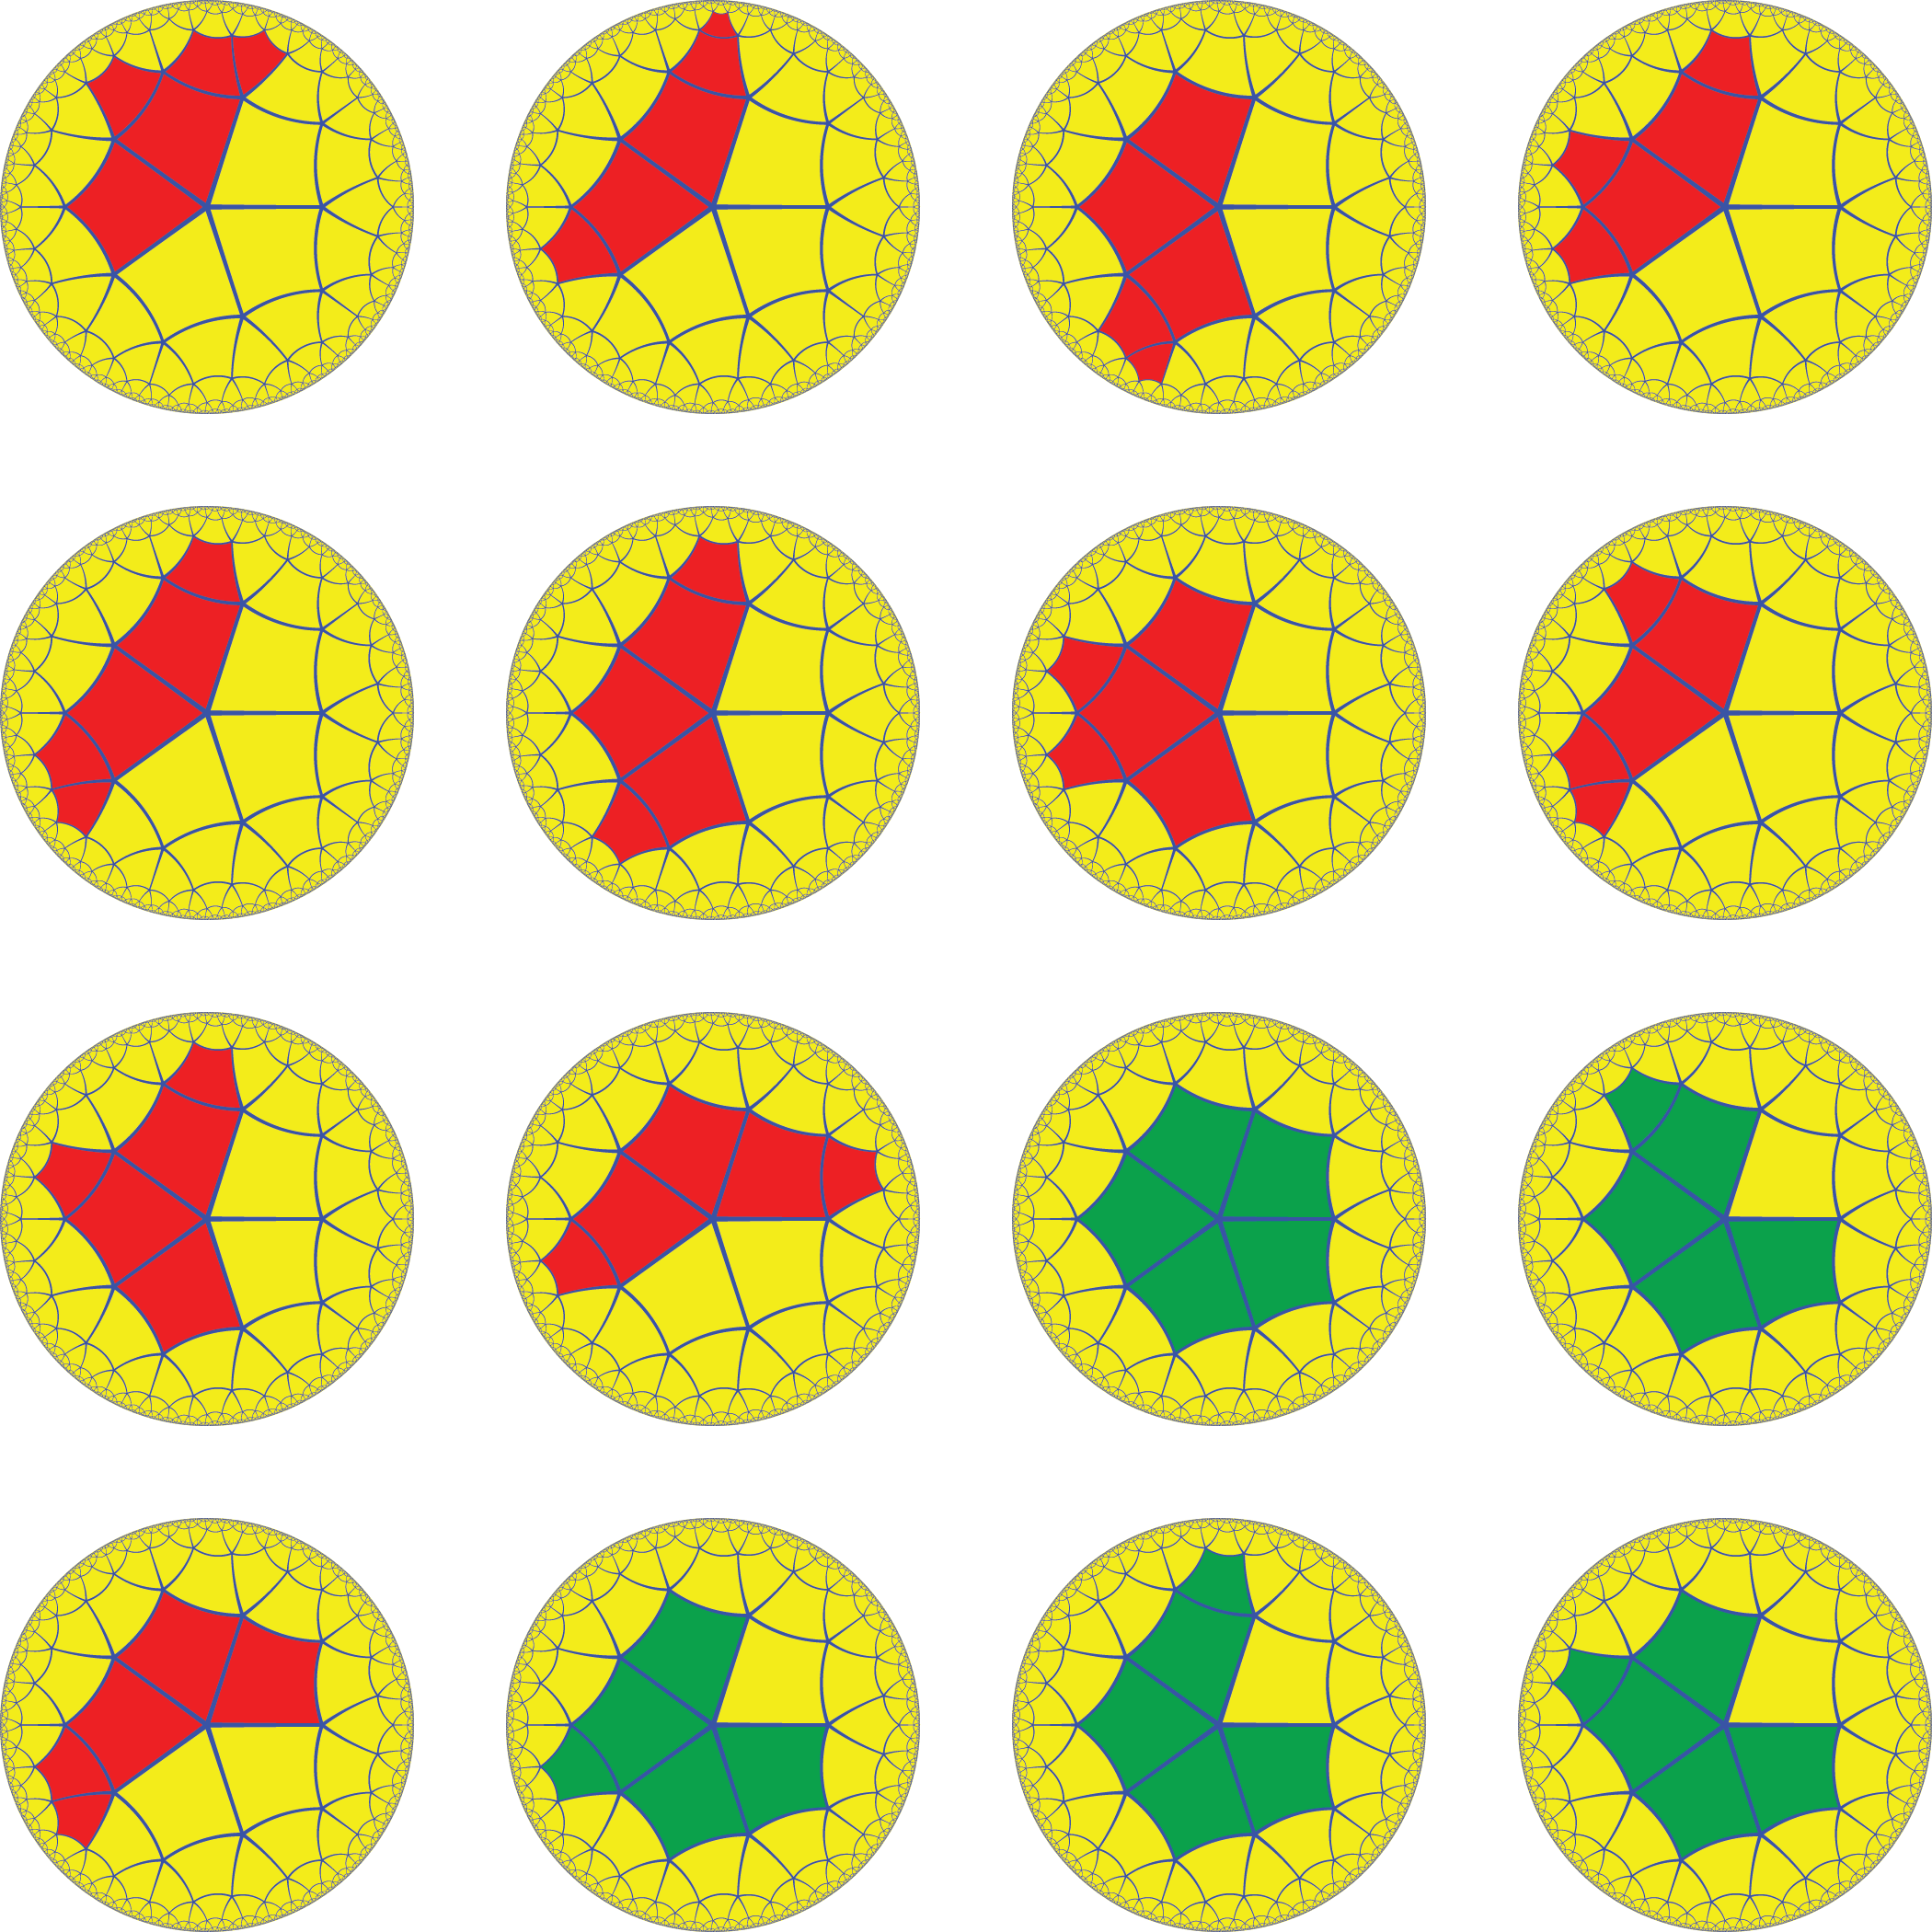
\includegraphics[scale=0.15]{assets/120_problem/5_4_hyperbolic_polyominoes.png}
  \caption{
    The $A119611(5)$ free pentominoes in the tessellation of the
    hyperbolic plane with Schl\"afli symbol $\{5,4\}$.
  }
\end{figure}

\begin{question}
  What is the asymptotic growth of $n_{\{p,k\}}$-form as a function of $n$,
  the number of cells?
\end{question}

\begin{related}
  \item Can this generalize to three or more dimensions the way polyominoes
  generalize to polycubes?
  \item Is there a meaningful notion of fixed vs 1-sided
    $\mathrm{poly}_{\{p,k\}}$-forms?
\end{related}


\begin{references}
  \item Problems 71, 72, 77, 101, 103, 108, and 109.
  \item \href{https://codegolf.stackexchange.com/q/200122/53884}{Code Golf Stack Exchange: Counting polyominoes on the hyperbolic plane.}
  \item \href{https://arxiv.org/abs/2109.05331}{arXiv: Extremal $\{p,q\}$-Animals}
\end{references}
\end{document}
